\documentclass[12pt]{article}
\usepackage[utf8]{inputenc}
\usepackage[T1,T2A]{fontenc}
\usepackage{graphicx}
\usepackage{csquotes}
\usepackage{amsmath}
\usepackage{amsthm}
\usepackage{hyperref}
\usepackage{amssymb}
\usepackage{listings}

\usepackage[ukrainian]{babel}

\lstset{
    basicstyle=\ttfamily\small,
    breaklines=true,
    commentstyle=\color{gray},
    keepspaces=true,
    numbers=left,
    numberstyle=\tiny,
    showstringspaces=false,
    breakatwhitespace=true,
    captionpos=b,
    frame=single
}

\author{Байбула Кирило Аленович}
\date{\today}

\title{Формальна верифікація системи “Платіжний термінал”}

\begin{document}
\maketitle

\section*{Імплементація}

Імплементація системи “Платіжний термінал” виконана на мові
програмування Dafny, яка підтримує формальну верифікацію коду та
редактор коду VS Code із відповідним розширенням “Dafny”. Система
складається з трьох основних класів та декількох допоміжних предикатів
для валідації даних.

\subsection*{Предикати валідації}

Предикати валідації необхідні в предумовах для валілації, у нашому
випадку, пін кода картки та її номера. Пін код має бути числом що
складається з чотирьох чисел, а номер картки з десяти в десятичній
репрезентації.

\begin{lstlisting}
predicate ValidPinCode(pin: nat)
{
  pin < 10000
}

predicate ValidCardId(id: nat)
{
  id > 0 && id < 100000000000 // 10-digit card ID 
}
\end{lstlisting}

\subsection*{Клас Card}

Зберігає вже провалідовані данні про картку, такі як:

\begin{itemize}
\item її номер
\item пін-код
\item баланс у центах
\item чи є вона заблокованою
\end{itemize}

\begin{lstlisting}
class Card {
  var id: nat
  var pinCode: nat
  var isBlocked: bool
  var balance: nat

  constructor(cardId: nat, pin: nat, blocked: bool, initialBalance: nat)
    requires ValidCardId(cardId)
    requires ValidPinCode(pin)
    ensures pinCode == pin
    ensures isBlocked == blocked
    ensures balance == initialBalance
    ensures id == cardId
  {
    id := cardId;
    pinCode := pin;
    isBlocked := blocked;
    balance := initialBalance;
  }
}
\end{lstlisting}

\subsection*{Клас TransactionData}

Данний клас зберігає інформацію про транзакцію: кількість в центах та
скільки на картці залишилося балансу.

\begin{lstlisting}
class TransactionData {
  var amount: nat  // Amount in cents
  var remainingBalance: nat  // Remaining balance in cents

  constructor(transAmount: nat, remBalance: nat)
    ensures amount == transAmount
    ensures remainingBalance == remBalance
  {
    amount := transAmount;
    remainingBalance := remBalance;
  }
}
\end{lstlisting}

\subsection*{Клас Terminal}

\begin{lstlisting}
class Terminal {
  var isConnectedToNetwork: bool
  var paper: nat // Length of left paper
  var authorizedUser: nat // Currently authorized user ID
  var lastTransactionData: TransactionData?

  constructor(connected: bool, paperLength: nat)
    ensures isConnectedToNetwork == connected
    ensures paper == paperLength
    ensures lastTransactionData == null
    ensures authorizedUser == 0
  {
    isConnectedToNetwork := connected;
    paper := paperLength;
    lastTransactionData := null;
    authorizedUser := 0;
  }
\end{lstlisting}

\subsubsection*{Клас Terminal: Функція Авторизації}

\begin{lstlisting}
  method Authorize(card: Card, enteredPin: nat) returns (success: bool)
    requires ValidPinCode(enteredPin)
    modifies this
    ensures !isConnectedToNetwork ==> !success
    ensures enteredPin != card.pinCode ==> !success
    ensures card.isBlocked ==> !success
    ensures isConnectedToNetwork && enteredPin == card.pinCode && !card.isBlocked ==> success
    ensures success ==> authorizedUser == card.id
  {
    success := false;  // Initialize with false by default

    if (!isConnectedToNetwork) {
      return;
    }

    if (enteredPin != card.pinCode) {
      return;
    }

    if (card.isBlocked) {
      return;
    }

    // All conditions are met
    success := true;
    authorizedUser := card.id;
  }
\end{lstlisting}

\subsubsection*{Клас Terminal: Функція Проведення транзакції}

\begin{lstlisting}
   method ProcessTransaction(card: Card, amount: nat) returns (success: bool)
    modifies this, card
    ensures !isConnectedToNetwork ==> !success
    ensures authorizedUser != card.id ==> !success
    ensures old(card.balance) < amount ==> !success
    ensures isConnectedToNetwork && authorizedUser == card.id && card.balance >= amount && amount >= 0 ==> success
    ensures success ==> card.balance == old(card.balance) - amount
    ensures success ==> lastTransactionData != null && lastTransactionData.amount == amount && lastTransactionData.remainingBalance == card.balance
    ensures !success ==> card.balance == old(card.balance)
  {
    success := false;  // Initialize with false by default

    if (!isConnectedToNetwork) {
      return;
    }

    if (authorizedUser != card.id) {
      return;
    }

    if (card.balance < amount) {
      return;
    }

    // All conditions are met
    card.balance := card.balance - amount;
    lastTransactionData := new TransactionData(amount, card.balance);
    success := true;
  }
\end{lstlisting}

\subsubsection*{Клас Terminal: Функція Проведення транзакції}

\begin{lstlisting}
   method PrintReceipt() returns (success: bool)
    modifies this
    ensures old(paper) == 0 ==> !success
    ensures old(lastTransactionData) == null ==> !success
    ensures paper > 0 && lastTransactionData != null ==> success
    ensures success ==> paper == old(paper) - 1
    ensures success ==> lastTransactionData == null
    ensures success ==> authorizedUser == 0
  {
    success := false;  // Initialize with false by default
    
    if (paper == 0) {
      return;
    }

    if (lastTransactionData == null) {
      return;
    }

    // All conditions are met
    paper := paper - 1; // Decrease paper length
    lastTransactionData := null; // Clear last transaction data
    authorizedUser := 0; // Reset authorized user
    success := true;
  }
\end{lstlisting}

\subsection*{Головна програма}

Для перевікри функціоналу було описану головний метод, що використовує
данний фукнціонал. У ньому було створено картку із номером
100,000,000, пінкодом 1234, початковим балансом 100000 центів та
статусом ``не заблокована''. Термін що під’єднаний до мережі та має
можливість роздрукувати п’ять чеків. Далі проходить авторизація,
проводиться транзакція в половину суми та друкується чек.

\begin{lstlisting}
method Main()
{
  print "Payment Terminal System Verification\n";

  var card := new Card(100_000_000, 1234, false, 100000);

  var terminal := new Terminal(true, 5);

  print "Testing Authorization...\n";
  var authSuccess := terminal.Authorize(card, 1234);
  print "Authorization ", if authSuccess then "succeeded" else "failed", "\n";

  print "Testing Transaction...\n";
  var transAmount: nat := 50000; // $500.00
  var transSuccess := terminal.ProcessTransaction(card, transAmount);

  print "Transaction for ", transAmount, " cents ", 
        if transSuccess then "succeeded" else "failed", "\n";

  if (transSuccess) {
    print "Remaining balance: ", card.balance, " cents\n";
  }

  print "Testing Receipt Printing...\n";
  var receiptSuccess := terminal.PrintReceipt();
  print "Receipt printing ", if receiptSuccess then "succeeded" else "failed", "\n";
  
  print "Verification complete!\n";
}
\end{lstlisting}

Запустивши команду \texttt{dafny run -t py Main.dfy} можна побачити,
що вся програма проверефікована і видає очікуваний результат:

\begin{figure}[h!]
  \centering
  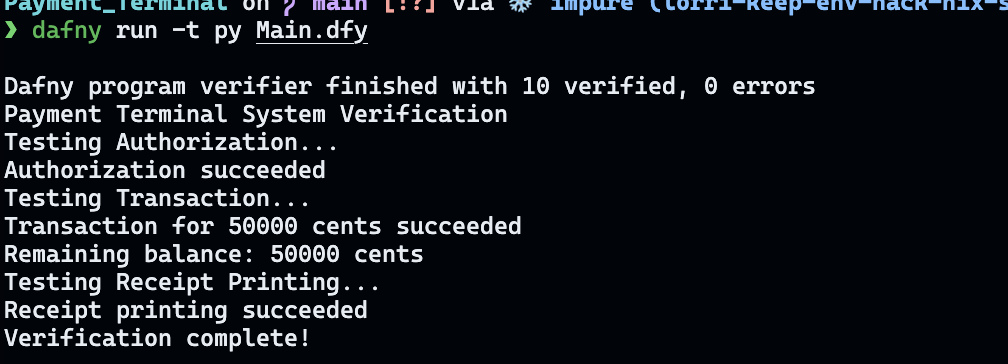
\includegraphics[scale=0.5]{dafny_run_result.png}
\end{figure}

\section*{Висновки}

Розроблена система демонструє використання формальних методів для
забезпечення коректності роботи платіжного терміналу мовою формальної
верифікації програм --- Dafny.

\end{document}
